\documentclass[tikz,convert={outfile=\jobname.svg}]{standalone}
\usetikzlibrary{arrows.meta}

% https://tex.stackexchange.com/questions/235525/how-to-write-these-symbols-double-vee-wedge-and-bracket
\usepackage{amsmath,stmaryrd}
\newcommand{\bigdoublewedge}{%
  \mathop{
    \mathchoice{\bigwedge\mkern-15mu\bigwedge}
               {\bigwedge\mkern-12.5mu\bigwedge}
               {\bigwedge\mkern-12.5mu\bigwedge}
               {\bigwedge\mkern-11mu\bigwedge}
    }
}
\newcommand{\bigdoublevee}{%
  \mathop{
    \mathchoice{\bigvee\mkern-15mu\bigvee}
               {\bigvee\mkern-12.5mu\bigvee}
               {\bigvee\mkern-12.5mu\bigvee}
               {\bigvee\mkern-11mu\bigvee}
    }
}

\begin{document}
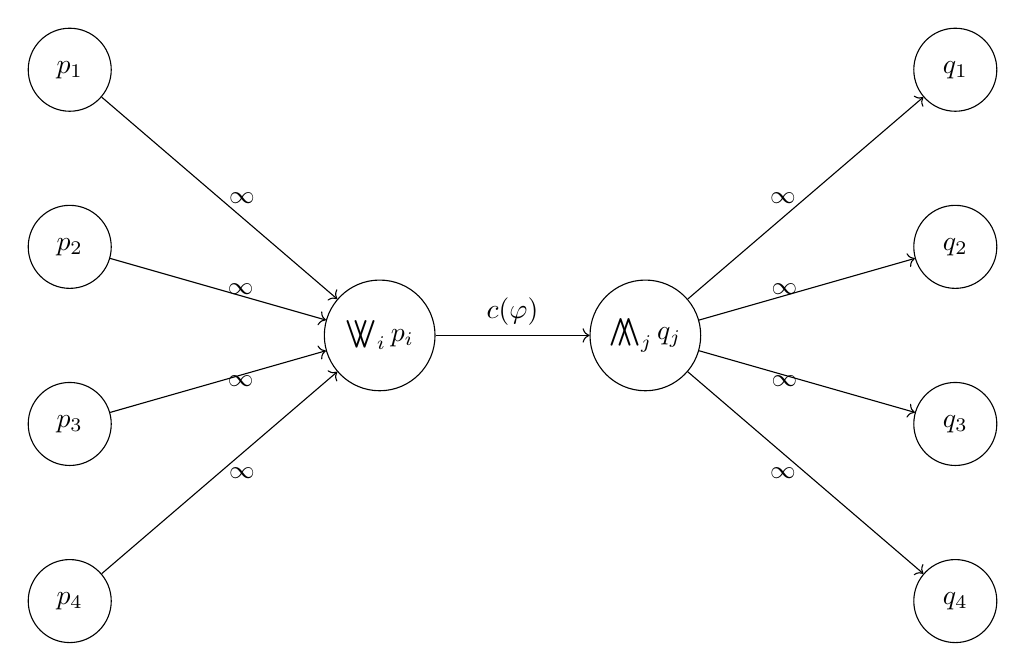
\begin{tikzpicture}[x=80pt, y=80pt]
    \node[draw=black, fill=white, circle, minimum size=30pt] at (-2,1.2) (p1) {$p_1$};
    \node[draw=black, fill=white, circle, minimum size=30pt] at (-2,0.4) (p2) {$p_2$};
    \node[draw=black, fill=white, circle, minimum size=30pt] at (-2,-0.4) (p3) {$p_3$};
    \node[draw=black, fill=white, circle, minimum size=30pt] at (-2,-1.2) (p4) {$p_4$};
    \node[draw=black, fill=white, circle, minimum size=30pt] at (2,1.2) (q1) {$q_1$};
    \node[draw=black, fill=white, circle, minimum size=30pt] at (2,0.4) (q2) {$q_2$};
    \node[draw=black, fill=white, circle, minimum size=30pt] at (2,-0.4) (q3) {$q_3$};
    \node[draw=black, fill=white, circle, minimum size=30pt] at (2,-1.2) (q4) {$q_4$};
    \node[draw=black, fill=white, circle, minimum size=40pt] at (-0.6,0) (p) {$\bigdoublevee_i p_i$};
    \node[draw=black, fill=white, circle, minimum size=40pt] at (0.6,0) (q) {$\bigdoublewedge_j q_j$};

    \draw[->] (p1) -- node[right] {\small $\infty$} (p);
    \draw[->] (p2) -- node[right] {\small $\infty$} (p);
    \draw[->] (p3) -- node[right] {\small $\infty$} (p);
    \draw[->] (p4) -- node[right] {\small $\infty$} (p);
    \draw[->] (p) -- node[above] {$c(\varphi)$} (q);
    \draw[->] (q) -- node[left] {\small $\infty$} (q1);
    \draw[->] (q) -- node[left] {\small $\infty$} (q2);
    \draw[->] (q) -- node[left] {\small $\infty$} (q3);
    \draw[->] (q) -- node[left] {\small $\infty$} (q4);
\end{tikzpicture}
\end{document}
